\section{Vector Algebra}

\subsection{Vector Magnitude}

\begin{definition}[Vector Magnitude]
  Let $\vec{v} = (v_1, v_2, v_3)$ be a vector in $\mathbb{E}^3$. The \textbf{magnitude} of $\vec{v}$ is defined as:
  \begin{equation}
    \|\vec{v}\| = \sqrt{v_1^2 + v_2^2 + v_3^2}
  \end{equation}
\end{definition}

\subsection{Vector Addition}

\begin{definition}[Vector Addition]
  Let $\vec{v} = (v_1, v_2, v_3)$ and $\vec{w} = (w_1, w_2, w_3)$ be vectors in $\mathbb{E}^3$. The \textbf{sum} of $\vec{v}$ and $\vec{w}$ is defined as:
  \begin{equation}
    \vec{v} + \vec{w} = (v_1 + w_1, v_2 + w_2, v_3 + w_3)
  \end{equation}
\end{definition}

Geometrically this can be seen as the {\bf diagonal} of a paralleleogram. Geometrically it is clear that you get the same effect as travelling along $\vec{v}$ and then $\vec{u}$

\begin{figure}[H]
\centering
   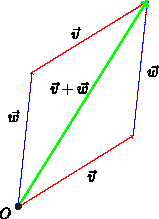
\includegraphics[scale=2.0]{vector_addition.pdf}
   \caption{Vector Addition} 
   \label{fig:figure-2-vector-addition}
\end{figure}

\clearpage

\subsubsection*{Vector Addition Properties}
\vspace{5px}
 
\begin{theorem}[Commutativity]
Suppose $\vec{v}$ and $\vec{w}$ be vectors in $\mathbb{E}^3$.\\
  If $\vec{v} = \left( v_1, v_2, v_3 \right)$ and $\vec{w} = \left(w_1, w_2, w_3 \right)$ be vectors in $\mathbb{E}^{3}$, then
  \begin{equation}
      \vec{v} + \vec{w} = \vec{w} + \vec{v}    
  \end{equation}
\end{theorem}
\begin{proof}
  Let $\vec{u}, \vec{v}, \vec{w}$ be vectors in $\mathbb{E}^3$. Then
  \begin{flalign*}
    \vec{v} + \vec{w} = \begin{bmatrix} v_1 \\ v_2 \\ v_3 \end{bmatrix} + \begin{bmatrix} w_1 \\ w_2 \\ w_3 \end{bmatrix} &=  \begin{bmatrix} v_1 + w_1 \\ v_2 + w_2 \\ v_3 + w_3 \end{bmatrix} &\\ \\
      &= \begin{bmatrix} w_1 + v_1 \\ w_2 + v_1 \\ w_3 + v_2 \end{bmatrix} \ \ \ \ \ \ \text{commutativity in } \mathbb{R}  &\\ \\ 
        &= \begin{bmatrix} w_1 \\ w_2 \\ w_3 \end{bmatrix}  + \begin{bmatrix} v_1 \\ v_2 \\ v_3 \end{bmatrix} = \vec{w} + \vec{v} &\\ 
  \end{flalign*}
\end{proof}

\begin{theorem}[Associativity]
  Suppose $\vec{u}$, $\vec{v}$ and $\vec{w}$ be vectors in $\mathbb{E}^3$.\\
  If $\vec{u} = \left( u_1, u_2, u_3 \right)$, $\vec{v} = \left(v_1, v_2, v_3 \right)$ and $\vec{w} = \left(w_1, w_2, w_3 \right)$ be vectors in $\mathbb{E}^{3}$, then
  \begin{equation}
    \vec{u} + \left( \vec{v} + \vec{w} \right) = \left( \vec{u} + \vec{v} \right) + \vec{w}
  \end{equation}
\end{theorem}
\begin{proof}
  Let $\vec{u}, \vec{v}, \vec{w}$ be vectors in $\mathbb{E}^3$. Then
  \begin{flalign*}
    \vec{u} + (\vec{v} + \vec{w}) = \begin{bmatrix} u_1 \\ u_2 \\ u_3 \end{bmatrix} + \Bigg(\begin{bmatrix} v_1 \\ v_2 \\ v_3 \end{bmatrix} \begin{bmatrix} w_1 \\ w_2 \\ w_3 \end{bmatrix} \Bigg) &=  \begin{bmatrix} u_1 + (v_1 + w_1) \\ u_2 + (v_2 + w_2) \\ u_3 + (v_3 + w_3) \end{bmatrix} &\\ \\
      &= \begin{bmatrix} (u_1 + v_1) + w_1 \\ (u_2 + w_2) + v_2 \\ (u_2 + v_3) + w_2 \end{bmatrix} \ \ \ \ \ \ \text{commutativity in } \mathbb{R}  &\\ \\ 
        &= \begin{bmatrix} u_1 + v_1  \\ u_1 + v_1 \\ u_1 + v_1 \end{bmatrix}  + \begin{bmatrix} w_1 \\ w_2 \\ w_3 \end{bmatrix} = (\vec{u} + \vec{v}) + \vec{w} &\\
 \end{flalign*} 
\end{proof}
\clearpage

\subsection{Scalar Multiplication}
Vectors can be multiplied by scalars to get a new vector. This is called \textbf{scalar multiplication}. The direction of the new vector depends on the sign of the scalar.
\begin{mycenter}
\tikzset{every picture/.style={line width=0.75pt}} %set default line width to 0.75pt        

\begin{tikzpicture}[x=0.75pt,y=0.75pt,yscale=-1,xscale=1]
%uncomment if require: \path (0,402); %set diagram left start at 0, and has height of 402
%Straight Lines [id:da7167353389209443] 
\draw    (252.21,236.82) -- (261.7,229.82) -- (279.26,216.3) ;
\draw [shift={(280.84,215.08)}, rotate = 142.4] [color={rgb, 255:red, 0; green, 0; blue, 0 }  ][line width=0.75]    (10.93,-3.29) .. controls (6.95,-1.4) and (3.31,-0.3) .. (0,0) .. controls (3.31,0.3) and (6.95,1.4) .. (10.93,3.29)   ;
%Straight Lines [id:da18547876587091028] 
\draw [color={rgb, 255:red, 208; green, 2; blue, 27 }  ,draw opacity=1 ]   (280.84,215.08) -- (336.51,172.81) ;
\draw [shift={(338.1,171.6)}, rotate = 142.79] [color={rgb, 255:red, 208; green, 2; blue, 27 }  ,draw opacity=1 ][line width=0.75]    (10.93,-3.29) .. controls (6.95,-1.4) and (3.31,-0.3) .. (0,0) .. controls (3.31,0.3) and (6.95,1.4) .. (10.93,3.29)   ;
%Straight Lines [id:da3504525720449021] 
\draw [color={rgb, 255:red, 208; green, 2; blue, 27 }  ,draw opacity=1 ]   (252.21,236.82) -- (196.54,279.09) ;
\draw [shift={(194.95,280.3)}, rotate = 322.79] [color={rgb, 255:red, 208; green, 2; blue, 27 }  ,draw opacity=1 ][line width=0.75]    (10.93,-3.29) .. controls (6.95,-1.4) and (3.31,-0.3) .. (0,0) .. controls (3.31,0.3) and (6.95,1.4) .. (10.93,3.29)   ;

% Text Node
\draw (261.7,229.82) node [anchor=north west][inner sep=0.75pt]   [align=left] {$\displaystyle \underline{v}$};
% Text Node
\draw (325,190) node [anchor=north west][inner sep=0.75pt]  [color={rgb, 255:red, 208; green, 2; blue, 27 }  ,opacity=1 ] [align=left] {$\displaystyle \lambda \underline{v}$ when $\displaystyle \lambda  >0$};
% Text Node
\draw (99,234) node [anchor=north west][inner sep=0.75pt]  [color={rgb, 255:red, 208; green, 2; blue, 27 }  ,opacity=1 ] [align=left] {$\displaystyle \lambda \underline{v}$ when $\displaystyle \lambda < 0$};

\end{tikzpicture}
\end{mycenter}

\begin{definition}[Scalar Multiplication]
  Let $\vec{v} = (v_1, v_2, v_3)$ be a vector in $\mathbb{E}^3$ and $\lambda \in \mathbb{R}$ be a scalar. The \textbf{scalar multiplication} of $\vec{v}$ and $\lambda$ is defined as:
  \begin{equation}
    \lambda \vec{v} = (\lambda v_1, \lambda v_2, \lambda v_3)
  \end{equation}
\end{definition}

\begin{tcolorbox}[title=Multiplying by a Scalar]
  Let $\vec{v}$ be a vector in $\mathbb{E}^3$ and $\lambda$ be a scalar. Then:
\begin{itemize}
  \item If $\lambda > 0$, then $\lambda \vec{v}$ is a vector in the same direction as $\vec{v}$ but with magnitude $\lambda \|\vec{v}\|$
  \item If $\lambda < 0$, then $\lambda \vec{v}$ is a vector in the opposite direction as $\vec{v}$ but with magnitude $|\lambda| \|\vec{v}\|$
\end{itemize}
\end{tcolorbox}

\subsubsection*{Scalar Multiplication Properties}
\vspace{5px}
\begin{theorem}[Distributivity over Scalar Multiplication]
 Let $\vec{u}$ and $\vec{v}$ be vectors in $\mathbb{E}^3$ and $\lambda$ be a scalar. Then
  \begin{equation}
    \lambda (\vec{u} + \vec{v}) = \lambda \vec{u} + \lambda \vec{v}
  \end{equation} 
\end{theorem}
\begin{proof}
  Let $\vec{u}, \vec{v} \in \mathbb{E}^{3}$
  \begin{flalign*}
    \lambda (\vec{u} + \vec{v}) = \lambda \begin{bmatrix} u_1 + v_1 \\ u_2 + v_2 \\ u_3 + v_3 \end{bmatrix} &= \begin{bmatrix} \lambda (u_1 + v_1) \\ \lambda (u_2 + v_2) \\ \lambda (u_3 + v_3) \end{bmatrix} &\\ \\
      &= \begin{bmatrix} \lambda u_1 + \lambda v_1 \\ \lambda u_2 + \lambda v_2 \\ \lambda u_3 + \lambda v_3 \end{bmatrix} = \begin{bmatrix} \lambda u_1 \\ \lambda u_2 \\ \lambda u_3 \end{bmatrix} + \begin{bmatrix} \lambda v_1 \\ \lambda v_2 \\ \lambda v_3 \end{bmatrix} = \lambda \vec{u} + \lambda \vec{v} &\\
  \end{flalign*}
\end{proof}
\clearpage

\begin{theorem}[Associativity]
  Let $\vec{v}$ be a vector in $\mathbb{E}^3$ and $\lambda, \mu$ be scalars. Then
  \begin{equation}
    (\lambda \mu) \vec{v} = \lambda (\mu \vec{v})
  \end{equation}
\end{theorem}
\begin{proof}
  Let $\vec{v} \in \mathbb{E}^{3}$
  \begin{flalign*}
    (\lambda \mu) \vec{v} = (\lambda \mu) \begin{bmatrix} v_1 \\ v_2 \\ v_3 \end{bmatrix} &= \begin{bmatrix} (\lambda \mu) v_1 \\ (\lambda \mu) v_2 \\ (\lambda \mu) v_3 \end{bmatrix} &\\ \\
      &= \begin{bmatrix} \lambda (\mu v_1) \\ \lambda (\mu v_2) \\ \lambda (\mu v_3) \end{bmatrix} = \lambda \begin{bmatrix} \mu v_1 \\ \mu v_2 \\ \mu v_3 \end{bmatrix} = \lambda (\mu \vec{v}) &\\
  \end{flalign*}
\end{proof}

\begin{theorem}[Distributivity over Vector Addition]
  Let $\vec{v}$ be a vector in $\mathbb{E}^3$ and $\lambda, \mu$ be scalars. Then
  \begin{equation}
    (\lambda + \mu) \vec{v} = \lambda \vec{v} + \mu \vec{v}
  \end{equation}
  
\end{theorem}
\begin{proof}
  Let $\vec{v}$ be a vector in $\mathbb{E}^{3}$
  \begin{flalign*}
    (\lambda + \mu) \vec{v} = (\lambda + \mu) \begin{bmatrix} v_1 \\ v_2 \\ v_3 \end{bmatrix} &= \begin{bmatrix} (\lambda + \mu) v_1 \\ (\lambda + \mu) v_2 \\ (\lambda + \mu) v_3 \end{bmatrix} &\\ \\
      &= \begin{bmatrix} \lambda v_1 + \mu v_1 \\ \lambda v_2 + \mu v_2 \\ \lambda v_3 + \mu v_3 \end{bmatrix} = \begin{bmatrix} \lambda v_1 \\ \lambda v_2 \\ \lambda v_3 \end{bmatrix} + \begin{bmatrix} \mu v_1 \\ \mu v_2 \\ \mu v_3 \end{bmatrix} = \lambda \vec{v} + \mu \vec{v} &\\
  \end{flalign*}
\end{proof}

\begin{theorem}[Identity]
  Let $\vec{v}$ be a vector in $\mathbb{E}^3$. Then
  \begin{equation}
    1 \vec{v} = \vec{v}
  \end{equation}
\end{theorem}
\begin{proof}
  Let $\vec{v}$ be a vector in $\mathbb{E}^{3}$
  \begin{flalign*}
    1 \vec{v} = 1 (v_1, v_2, v_3) &=  (1v_1, 1v_2, 1 v_3) &\\ \\
    &= (v_1, v_2, v_3) = \vec{v} &\\
  \end{flalign*}
\end{proof}

\clearpage

\subsection{Vector Subtraction}
\begin{definition}[Vector Subtraction]
  Let $\vec{v}$ and $\vec{w}$ be vectors in $\mathbb{E}^3$. The \textbf{difference} of $\vec{v}$ and $\vec{w}$ is defined as:
  \begin{equation}
    \vec{v} - \vec{w} = \vec{v} + (-1) \vec{w}
  \end{equation}
\end{definition}
Geometrically we can see this in the following diagram:
\begin{figure}[H]

\centering
\begin{tikzpicture}[x=0.75pt,y=0.75pt,yscale=-1,xscale=1]
%uncomment if require: \path (0,402); %set diagram left start at 0, and has height of 402

%Straight Lines [id:da8907486632779575] 
\draw [color={rgb, 255:red, 80; green, 227; blue, 194 }  ,draw opacity=1 ]   (289,170) -- (397.9,144.97) ;
\draw [shift={(399.85,144.53)}, rotate = 167.06] [color={rgb, 255:red, 80; green, 227; blue, 194 }  ,draw opacity=1 ][line width=0.75]    (10.93,-3.29) .. controls (6.95,-1.4) and (3.31,-0.3) .. (0,0) .. controls (3.31,0.3) and (6.95,1.4) .. (10.93,3.29)   ;
%Straight Lines [id:da39975023073176996] 
\draw [color={rgb, 255:red, 208; green, 2; blue, 27 }  ,draw opacity=1 ]   (289,170) -- (345.79,53.39) ;
\draw [shift={(346.67,51.59)}, rotate = 115.97] [color={rgb, 255:red, 208; green, 2; blue, 27 }  ,draw opacity=1 ][line width=0.75]    (10.93,-3.29) .. controls (6.95,-1.4) and (3.31,-0.3) .. (0,0) .. controls (3.31,0.3) and (6.95,1.4) .. (10.93,3.29)   ;
%Straight Lines [id:da469577497474827] 
\draw [color={rgb, 255:red, 74; green, 144; blue, 226 }  ,draw opacity=1 ] [dash pattern={on 4.5pt off 4.5pt}]  (289,170) -- (180.1,195.03) ;
\draw [shift={(178.15,195.47)}, rotate = 347.06] [color={rgb, 255:red, 74; green, 144; blue, 226 }  ,draw opacity=1 ][line width=0.75]    (10.93,-3.29) .. controls (6.95,-1.4) and (3.31,-0.3) .. (0,0) .. controls (3.31,0.3) and (6.95,1.4) .. (10.93,3.29)   ;
%Straight Lines [id:da1613229280153815] 
\draw [color={rgb, 255:red, 208; green, 2; blue, 27 }  ,draw opacity=1 ] [dash pattern={on 4.5pt off 4.5pt}]  (231.33,288.41) -- (288.12,171.8) ;
\draw [shift={(289,170)}, rotate = 115.97] [color={rgb, 255:red, 208; green, 2; blue, 27 }  ,draw opacity=1 ][line width=0.75]    (10.93,-3.29) .. controls (6.95,-1.4) and (3.31,-0.3) .. (0,0) .. controls (3.31,0.3) and (6.95,1.4) .. (10.93,3.29)   ;
%Straight Lines [id:da43055619556326463] 
\draw [color={rgb, 255:red, 245; green, 166; blue, 35 }  ,draw opacity=1 ] [dash pattern={on 0.84pt off 2.51pt}]  (231.33,288.41) -- (179.14,197.21) ;
\draw [shift={(178.15,195.47)}, rotate = 60.22] [color={rgb, 255:red, 245; green, 166; blue, 35 }  ,draw opacity=1 ][line width=0.75]    (10.93,-3.29) .. controls (6.95,-1.4) and (3.31,-0.3) .. (0,0) .. controls (3.31,0.3) and (6.95,1.4) .. (10.93,3.29)   ;
%Straight Lines [id:da15370302119538037] 
\draw [color={rgb, 255:red, 245; green, 166; blue, 35 }  ,draw opacity=1 ]   (289,170) -- (236.81,78.8) ;
\draw [shift={(235.82,77.07)}, rotate = 60.22] [color={rgb, 255:red, 245; green, 166; blue, 35 }  ,draw opacity=1 ][line width=0.75]    (10.93,-3.29) .. controls (6.95,-1.4) and (3.31,-0.3) .. (0,0) .. controls (3.31,0.3) and (6.95,1.4) .. (10.93,3.29)   ;

% Text Node
\draw (305,73) node [anchor=north west][inner sep=0.75pt]  [color={rgb, 255:red, 208; green, 2; blue, 27 }  ,opacity=1 ] [align=left] {$\displaystyle \underline{v}$};
% Text Nodedocker
\draw (344.43,157.26) node [anchor=north west][inner sep=0.75pt]  [color={rgb, 255:red, 80; green, 227; blue, 194 }  ,opacity=1 ] [align=left] {$\displaystyle \underline{u}$};
% Text Node
\draw (214.43,153.26) node [anchor=north west][inner sep=0.75pt]  [color={rgb, 255:red, 74; green, 144; blue, 226 }  ,opacity=1 ] [align=left] {$\displaystyle -\underline{u}$};
% Text Node
\draw (268,215) node [anchor=north west][inner sep=0.75pt]  [color={rgb, 255:red, 208; green, 2; blue, 27 }  ,opacity=1 ] [align=left] {$\displaystyle \underline{v}$};
% Text Node
\draw (151,245) node [anchor=north west][inner sep=0.75pt]  [color={rgb, 255:red, 245; green, 166; blue, 35 }  ,opacity=1 ] [align=left] {$\displaystyle \underline{v} \ -\ \underline{u}$};
% Text Node
\draw (204,105) node [anchor=north west][inner sep=0.75pt]  [color={rgb, 255:red, 245; green, 166; blue, 35 }  ,opacity=1 ] [align=left] {$\displaystyle \underline{v} \ -\ \underline{u}$};

\end{tikzpicture}
\end{figure}

\subsection{Unit Vectors}
\begin{definition}[Unit Vector]
  A \textbf{unit vector} is a vector with magnitude 1. The unit vector in the {\bf direction} of $\vec{v}$ is denoted by $\hat{v}$.
  Unit vector is calculated by:
  \begin{equation}
    \hat{v} = \frac{\vec{v}}{\|\vec{v}\|}
  \end{equation}
\end{definition}

